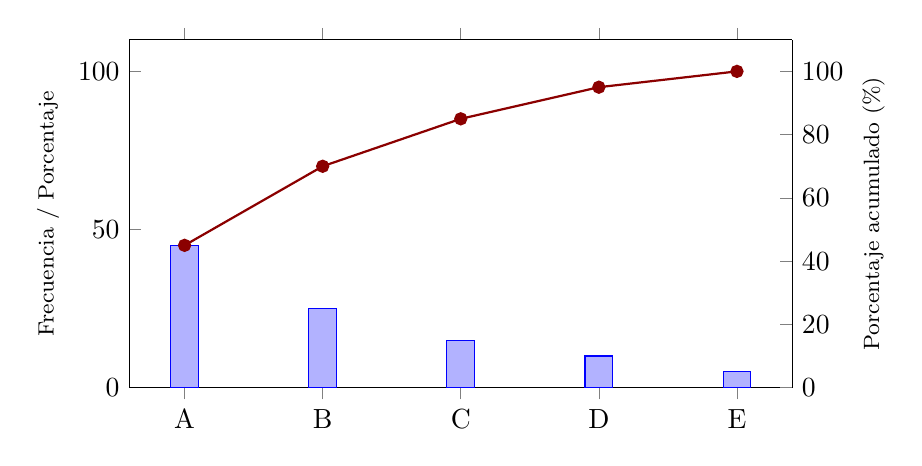
\begin{tikzpicture}
  \begin{axis}[
      width=10cm,height=6cm,
      ybar,ymin=0,ymax=110,
      axis y line*=left,
      ylabel={\footnotesize Frecuencia / Porcentaje},
      symbolic x coords={A, B, C, D, E},
      xtick=data
    ]
    \addplot coordinates {(A,45) (B,25) (C,15) (D,10) (E,5)};
  \end{axis}

  \begin{axis}[
      width=10cm,height=6cm,
      ymin=0,ymax=110,
      axis y line*=right,
      ytick={0,20,40,60,80,100},
      ylabel={\footnotesize Porcentaje acumulado (\%)},
      axis x line=none,
      symbolic x coords={A, B, C, D, E},
      xtick=data
    ]
    \addplot[DarkRed, thick, mark=*] coordinates {(A,45) (B,70) (C,85) (D,95) (E,100)};
  \end{axis}
\end{tikzpicture}